\usetikzlibrary{decorations.pathmorphing}
\usetikzlibrary{decorations.markings}
\usetikzlibrary{decorations.pathmorphing}
\usetikzlibrary{arrows}
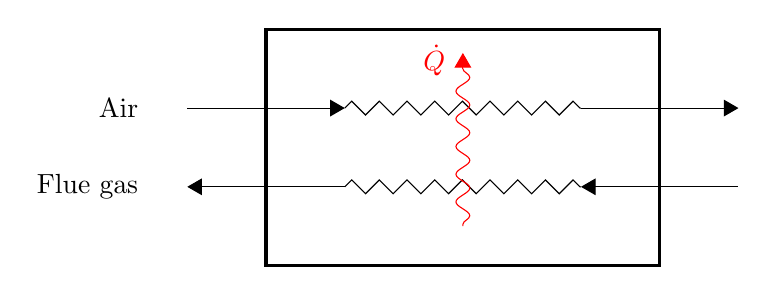
\begin{tikzpicture}[>=triangle 60]
% rectangle
\draw[very thick] (0,0) rectangle (5,3);
% air line
\draw[->]  (-1,2)--(1,2);
\draw[decorate,decoration=zigzag] (1,2)--(4,2);
\draw[->]  (4,2)--(6,2);
% flue gas linetriangle 60
\draw[<-]  (-1,1)--(1,1);
\draw[decorate,decoration=zigzag] (1,1)--(4,1);
\draw[<-]  (4,1)--(6,1);
%
\node[left] at (-1.5,2) {Air};
\node[left] at (-1.5,1) {Flue gas};
% heat transfer
\draw[red, decorate,decoration=snake] (2.5,2.5)--(2.5,0.5);
\draw[red,->]  (2.5,2.5)--(2.5,2.7);
\node[red,left] at (2.4,2.6) {$\dot{Q}$};
\end{tikzpicture}